\documentclass[a4paper,12pt]{article}

\textwidth 17cm \textheight 25cm \evensidemargin 0cm
\oddsidemargin 0cm \topmargin -2cm
\parindent 0pt
%\parskip \bigskipamount

\usepackage{graphicx}
\usepackage[dutch]{babel}
\usepackage{amssymb,amsthm,amsmath}
%\usepackage{dot2texi}
\usepackage[utf8]{inputenc}
\usepackage{nopageno}
\usepackage{pdfpages}
\usepackage{enumerate}
\usepackage{caption}
\usepackage{wrapfig}
\usepackage{pgf,tikz,pgfplots}
\pgfplotsset{compat=1.15}
\usepackage{color}
\usetikzlibrary{arrows}
\usetikzlibrary{patterns}
\usepackage{fancyhdr}
\pagestyle{fancy}
\usepackage[version=3]{mhchem}
\usepackage{multicol}
\usepackage{fix-cm}
\usepackage{setspace}
\usepackage{mhchem}
\usepackage{xhfill}
\usepackage{parskip}
\usepackage{cancel}
\usepackage{mdframed}
\usepackage{url}
\usepackage{mathtools}
\usepackage{changepage}

\newcommand{\todo}[1]{{\color{red} TODO: #1}}

\newcommand{\degree}{\ensuremath{^\circ}}
\newcommand\rad{\qopname\relax o{\mathrm{rad}}}

\newcommand\ggd{\qopname\relax o{\mathrm{ggd}}}

\pgfmathdeclarefunction{gauss}{2}{%
  \pgfmathparse{1/(#2*sqrt(2*pi))*exp(-((x-#1)^2)/(2*#2^2))}%
}

\def\LRA{\Leftrightarrow}

\newcommand{\zrmbox}{\framebox{\phantom{EXE}}\phantom{X}}
\newcommand{\zrm}[1]{\framebox{#1}}

% environment oefening:
% houdt een teller bij die de oefeningen nummert, probeert ook de oefening op één pagina te houden
\newcounter{noefening}
\setcounter{noefening}{0}
\newenvironment{oefening}
{
  \stepcounter{noefening}
  \pagebreak[0]
  \begin{minipage}{\textwidth}
  \vspace*{0.7cm}{\large\bf Oefening \arabic{noefening}}
}{%
  \end{minipage}
}

\usepackage{calc}

% vraag
\reversemarginpar
\newcounter{punten}
\setcounter{punten}{0}
\newcounter{nvraag}
\setcounter{nvraag}{1}
\newlength{\puntwidth}
\newlength{\boxwidth}
\newcommand{\vraag}[1]{
\settowidth{\puntwidth}{\Large{#1}}
\setlength{\boxwidth}{1.5cm}
\addtolength{\boxwidth}{-\puntwidth}
{\large\bf Vraag \arabic{nvraag} \addtocounter{nvraag}{1}}\vspace*{-0.5cm}
{\marginpar{\color{lightgray}\fbox{\parbox{1.5cm}{\vspace*{1cm}\hspace*{\boxwidth}{\Large{#1}}}}}
\vspace*{0.5cm}}
\addtocounter{punten}{#1}}

% arulefill
\def\arulefill{\leavevmode{\xrfill[-5pt]{0.3pt}[lightgray]\endgraf}\vspace*{0.2cm}}

% \arules{n}
\newcommand{\arules}[1]{
\color{lightgray}
%\vspace*{0.05cm}
\foreach \n in {1,...,#1}{
  \vspace*{0.75cm}
  \hrule height 0.3pt\hfill
}\color{black}\vspace*{0.2cm}}

% \arule{x}
\newcommand{\arule}[1]{
\color{lightgray}{\raisebox{-0.1cm}{\rule[-0.05cm]{#1}{0.3pt}}}\color{black}
}

% \abox{y}
\newcommand{\abox}[1]{
\fbox{
\begin{minipage}{\textwidth- 4\fboxsep}
\hspace*{\textwidth}\vspace{#1}
\end{minipage}
}
}

\newcommand{\ruitjes}[1]{
\definecolor{cqcqcq}{rgb}{0.85,0.85,0.85}
\hspace*{-2.5cm}
\begin{tikzpicture}[scale=1.04,line cap=round,line join=round,>=triangle 45,x=1.0cm,y=1.0cm]
\draw [color=cqcqcq, xstep=0.5cm, ystep=0.5cm] (0,-#1) grid (20.5,0);
\end{tikzpicture}
}


\newcommand{\assenstelsel}[5][1]{
\definecolor{cqcqcq}{rgb}{0.65,0.65,0.65}
\begin{tikzpicture}[line cap=round,line join=round,>=triangle 45,x=#1cm,y=#1cm]
\draw [color=cqcqcq,dash pattern=on 1pt off 1pt, xstep=1.0cm,ystep=1.0cm] (#2,#4) grid (#3,#5);
\draw[->,color=black] (#2,0) -- (#3,0);
%\draw[shift={(1,0)},color=black] (0pt,2pt) -- (0pt,-2pt) node[below] {\footnotesize $1$};
%\draw[color=black] (#3.25,0.07) node [anchor=south west] {$x$};
\draw[->,color=black] (0,#4) -- (0,#5);
%\draw[shift={(0,1)},color=black] (2pt,0pt) -- (-2pt,0pt) node[left] {\footnotesize $1$};
\draw[color=black] (0.09,#5.25) node [anchor=west] {\phantom{$y$}};
%\draw[color=black] (0pt,-10pt) node[right] {\footnotesize $0$};
\end{tikzpicture}
}

\newcommand{\getallenas}[3][1]{
\definecolor{cqcqcq}{rgb}{0.65,0.65,0.65}
\begin{tikzpicture}[scale=#1,line cap=round,line join=round,>=triangle 45,x=1.0cm,y=1.0cm]
\draw [color=cqcqcq,dash pattern=on 1pt off 1pt, xstep=1.0cm,ystep=1.0cm] (#2,-0.2) grid (#3,0.2);
\draw[->,color=black] (#2.25,0) -- (#3.5,0);
\draw[shift={(0,0)},color=black] (0pt,2pt) -- (0pt,-2pt) node[below] {\footnotesize $0$};
\draw[shift={(1,0)},color=black] (0pt,2pt) -- (0pt,-2pt) node[below] {\footnotesize $1$};
\draw[color=black] (#3.25,0.07) node [anchor=south west] {$\mathbb{R}$};
\end{tikzpicture}
}

\newcommand{\visgraad}[1]{\begin{tabular}{p{0.5cm}|p{#1}}&\\\hline\\\end{tabular}}

\newcommand{\tekenschema}[2]{\begin{tabular}{p{0.5cm}|p{#1}}&\\\hline\\[#2]\end{tabular}}

% schema van Horner
\newcommand{\schemahorner}{
\begin{tabular}{p{0.5cm}|p{7cm}}
&\\[1.5cm]
\hline\\
\end{tabular}}

% geef tabular iets meer ruimte
\setlength{\tabcolsep}{14pt}
\renewcommand{\arraystretch}{1.5}

\newcommand{\toets}[3]{
\thispagestyle{plain}
\vspace*{-2.5cm}
\begin{tikzpicture}[remember picture, overlay]
    \node [shift={(15.25 cm,-1.6cm)}] {%
        \includegraphics[width=1.8cm]{/home/ppareit/kaa1415/logokaavelgem.png}%
    };%
\end{tikzpicture}

\begin{tabular}{|llc|c|}
\hline
\vspace*{-0.5cm}
&&&\\
Naam & \arule{4cm} & {\Large\bf KA AVELGEM} & \\
\vspace*{-0.75cm}
&&&\\
Klas & \arule{4cm} & {\Large\bf 20...-...-...} & \\
\hline
\vspace*{-0.75cm}
&&&\\
Toets & {\bf #2} & {\large\bf #1} & Beoordeling\\
\vspace*{-0.75cm}
&&&\\
Onderwerp & \multicolumn{2}{l|}{\bf #3} &\\
\hline
\end{tabular}
}

\newcommand{\oefeningen}[1]{

\fancyhead[LE, RO]{\vspace{0.5cm} #1}
%\thispagestyle{plain}

{\bf \Large \centering Oefeningen: #1}

}

\raggedbottom

\newcommand\vl{\qopname\relax o{\mathrm{vl}}}

\newcommand\dom{\qopname\relax o{\mathrm{dom}}}
\newcommand\ber{\qopname\relax o{\mathrm{ber}}}

\newcommand\mC{\qopname\relax o{\mathrm{mC}}}
\newcommand\uC{\qopname\relax o{\mathrm{{\mu}C}}}
\newcommand\C{\qopname\relax o{\mathrm{C}}}

\newcommand\W{\qopname\relax o{\mathrm{W}}}
\newcommand\kW{\qopname\relax o{\mathrm{kW}}}
\newcommand\kWh{\qopname\relax o{\mathrm{kWh}}}


\newcommand\V{\qopname\relax o{\mathrm{V}}}
\newcommand\ohm{\qopname\relax o{\mathrm{\Omega}}}
\newcommand\kohm{\qopname\relax o{\mathrm{k\Omega}}}


\newcommand\N{\qopname\relax o{\mathrm{N}}}

\newcommand\Nperkg{\qopname\relax o{\mathrm{N/kg}}}

\newcommand\Nperm{\qopname\relax o{\mathrm{N/m}}}

\newcommand\gpermol{\qopname\relax o{\mathrm{g/mol}}}


\newcommand\kgperm{\qopname\relax o{\mathrm{kg/m}}}
\newcommand\kgperdm{\qopname\relax o{\mathrm{kg/dm}}}
\newcommand\gpercm{\qopname\relax o{\mathrm{g/cm}}}
\newcommand\gperml{\qopname\relax o{\mathrm{g/ml}}}


\newcommand{\mA}{\;\mbox{mA}}
\newcommand{\A}{\;\mbox{A}}
\newcommand{\MA}{\;\mbox{MA}}

\newcommand{\us}{\;\mu\mbox{s}}
\newcommand\s{\qopname\relax o{\mathrm{s}}}

\newcommand\h{\qopname\relax o{\mathrm{h}}}

\newcommand{\kmperh}{\;\mbox{km/h}}
\newcommand{\mpers}{\;\mbox{m/s}}
\newcommand{\kmpermin}{\;\mbox{km/min}}
\newcommand{\kmpers}{\;\mbox{km/s}}

\newcommand{\mph}{\;\mbox{mph}}

\newcommand{\Hz}{\;\mbox{Hz}}

\newcommand\Gm{\qopname\relax o{\mathrm{Gm}}}
\newcommand\Mm{\qopname\relax o{\mathrm{Mm}}}
\newcommand\km{\qopname\relax o{\mathrm{km}}}
\newcommand\hm{\qopname\relax o{\mathrm{hm}}}
\newcommand\dam{\qopname\relax o{\mathrm{dam}}}
\newcommand\m{\qopname\relax o{\mathrm{m}}}
\newcommand\dm{\qopname\relax o{\mathrm{dm}}}
\newcommand\cm{\qopname\relax o{\mathrm{cm}}}
\newcommand\mm{\qopname\relax o{\mathrm{mm}}}
\newcommand\um{\qopname\relax o{\mathrm{{\mu}m}}}
\newcommand\nm{\qopname\relax o{\mathrm{nm}}}


\newcommand\Gg{\qopname\relax o{\mathrm{Gg}}}
\newcommand\Mg{\qopname\relax o{\mathrm{Mg}}}
\newcommand\kg{\qopname\relax o{\mathrm{kg}}}
\newcommand\hg{\qopname\relax o{\mathrm{hg}}}
\renewcommand\dag{\qopname\relax o{\mathrm{dag}}}
\newcommand\g{\qopname\relax o{\mathrm{g}}}
\newcommand\dg{\qopname\relax o{\mathrm{dg}}}
\newcommand\cg{\qopname\relax o{\mathrm{cg}}}
\newcommand\mg{\qopname\relax o{\mathrm{mg}}}
\newcommand\ug{\qopname\relax o{\mathrm{{\mu}g}}}
\renewcommand\ng{\qopname\relax o{\mathrm{ng}}}

\newcommand\ton{\qopname\relax o{\mathrm{ton}}}

\newcommand\Gl{\qopname\relax o{\mathrm{Gl}}}
\newcommand\Ml{\qopname\relax o{\mathrm{Ml}}}
\newcommand\kl{\qopname\relax o{\mathrm{kl}}}
\newcommand\hl{\qopname\relax o{\mathrm{hl}}}
\newcommand\dal{\qopname\relax o{\mathrm{dal}}}
\renewcommand\l{\qopname\relax o{\mathrm{l}}}
\newcommand\dl{\qopname\relax o{\mathrm{dl}}}
\newcommand\cl{\qopname\relax o{\mathrm{cl}}}
\newcommand\ml{\qopname\relax o{\mathrm{ml}}}
\newcommand\ul{\qopname\relax o{\mathrm{{\mu}l}}}
\newcommand\nl{\qopname\relax o{\mathrm{nl}}}

\newcommand\MJ{\qopname\relax o{\mathrm{MJ}}}
\newcommand\kJ{\qopname\relax o{\mathrm{kJ}}}
\newcommand\J{\qopname\relax o{\mathrm{J}}}

\newcommand\T{\qopname\relax o{\mathrm{T}}}
\newcommand\uT{\qopname\relax o{\mathrm{{\mu}T}}}

\newcommand\grC{\qopname\relax o{\mathrm{{\degree}C}}}

\newcommand\K{\qopname\relax o{\mathrm{K}}}
\newcommand\calperK{\qopname\relax o{\mathrm{cal/K}}}

\newcommand\hPa{\qopname\relax o{\mathrm{hPa}}}
\newcommand\Pa{\qopname\relax o{\mathrm{Pa}}}

\newcommand\dB{\qopname\relax o{\mathrm{dB}}}

\newcommand\Var{\qopname\relax o{\mathrm{Var}}}

\newcommand{\EE}[1]{\cdot 10^{#1}}

\onehalfspacing

%\setlength{\headsep}{0cm}

\newenvironment{exlist}[1] %
{ \begin{multicols}{#1}
  \begin{enumerate}[(a)]
    \setlength{\itemsep}{0.5em} }
{ \end{enumerate}
  \end{multicols} }




\begin{document}

\thispagestyle{empty}
\begin{center}
  \begin{mdframed}
  \centering
  \fontsize{40}{50}\selectfont Goniometrische formules
  \end{mdframed}
  \vfill
  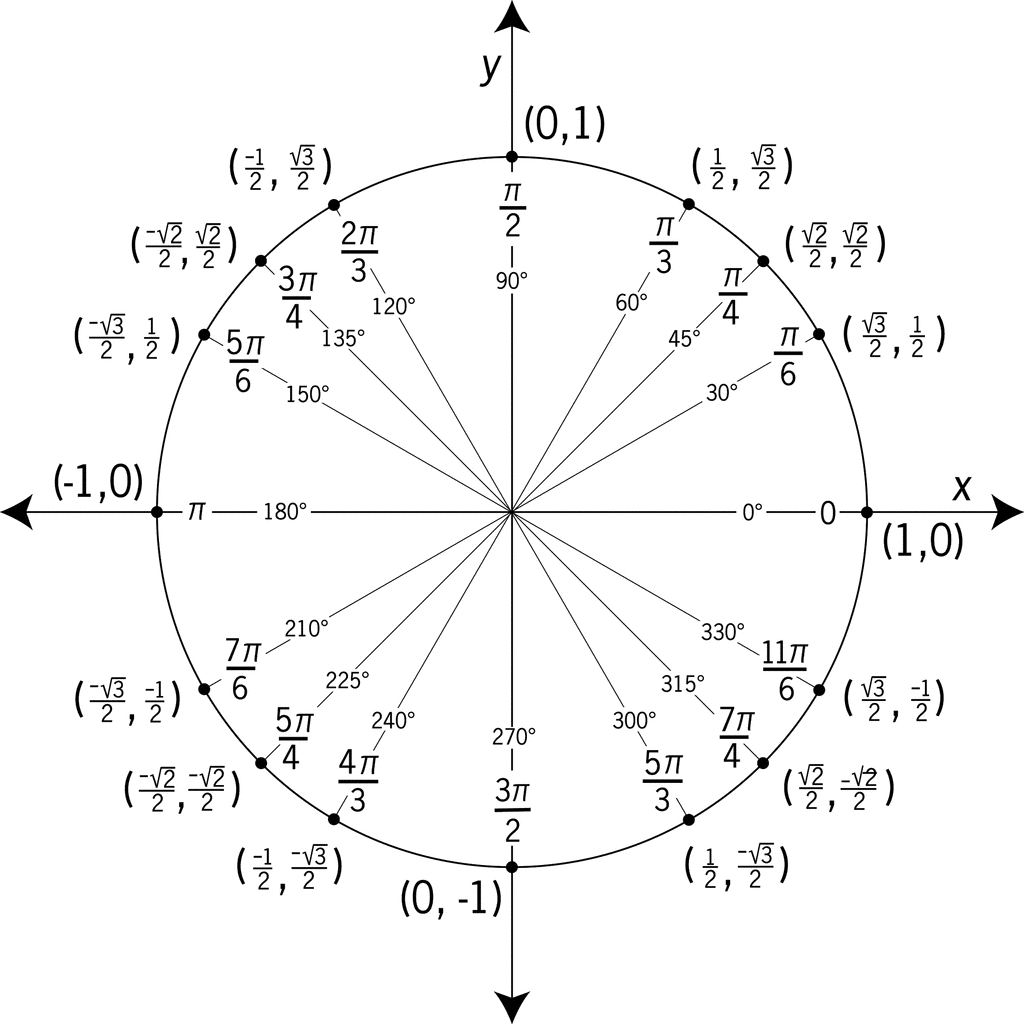
\includegraphics[width=0.7\textwidth]{unit-circle}
  \vfill
\end{center}
\subsection*{Doelstelling}
Je \hfill  {\scriptsize(LP 2006-059, LI 1.6.3)}
\begin{itemize}
  \item kan de optellingsformules voor sinus, cosinus en tangens opstellen en toepassen
  \item de verdubbelingsformules voor sinus, cosinus en tangens opstellen en toepassen
  \item de halveringsformules voor sinus en cosinus opstellen en toepassen
  \item de formules van Simpson opstellen en toepassen
\end{itemize}


\pagestyle{empty}
\mbox{}
\newpage
\clearpage
\thispagestyle{empty}
%\mbox{}
\tableofcontents
\newpage
\clearpage
\pagenumbering{arabic} 

\pagestyle{fancy}
\lhead{}
\rhead{Goniometrische formules}

\onehalfspacing

\section{Goniometrische getallen}

Voor een hoek met maatgetal $\alpha$ en beeldpunt $\vec{p}=(p_x,p_y)$ op de goniometrische cirkel definiëren we de goniometrische getallen als volgt:

\begin{itemize}
  \item De {\bf cosinus} van $\alpha$ is de $x$-coördinaat van $\vec{p}$: $\cos\alpha=p_x$
  \item De {\bf sinus} van $\alpha$ is de $y$-coördinaat van $\vec{p}$: $\cos\alpha=p_y$
\end{itemize}

Merk op:
\begin{itemize}
  \item De goniometrische getallen liggen in het interval $[-1,1]$.
  \item De goniometrische getallen hangen slechts van de hoek af en niet van zijn maatgetal, m.a.w.
  $$\alpha = \alpha + k\cdot 360\degree\mbox{ met }k\in\mathbb{Z}$$
\end{itemize}

Door stelling van Pythagoras toe te passen vinden we de {\bf grondformule van de goniometrie}
$$\cos^2\alpha + \sin^2\alpha = 1$$

Verder worden nog volgende afgeleide goniometrische getallen gedefinieerd:
\begin{itemize}
  \item De {\bf tangens} van $\alpha$:
  $$\tan\alpha=\dfrac{\sin\alpha}{\cos\alpha}$$
  \item De {\bf cotangens} van $\alpha$:
  $$\cot\alpha=\dfrac{\cos\alpha}{\sin\alpha}$$
  \item De {\bf secans} van $\alpha$:
  $$\sec\alpha=\dfrac{1}{\cos\alpha}$$
  \item De {\bf cosecans} van $\alpha$:
  $$\csc\alpha=\dfrac{1}{\cos\alpha}$$
\end{itemize}

\pagebreak
\section{Goniometrische getallen van enkele bijzondere hoeken}
\begin{center}
  \begin{tabular}{c|c|c|c|c|c|c|c|c|c}
    $x$ & $0\degree$ & $30\degree$ & $45\degree$ & $60\degree$ & $90\degree$ & $120\degree$ & $135\degree$ & $150\degree$ & $180\degree$ \\
    \hline
    $\sin x$&&&&&&&&&\\
    \hline
    $\cos x$&&&&&&&&&\\
    \hline
    $\tan x$&&&&&&&&&\\ 
  \end{tabular}
  \vfill
  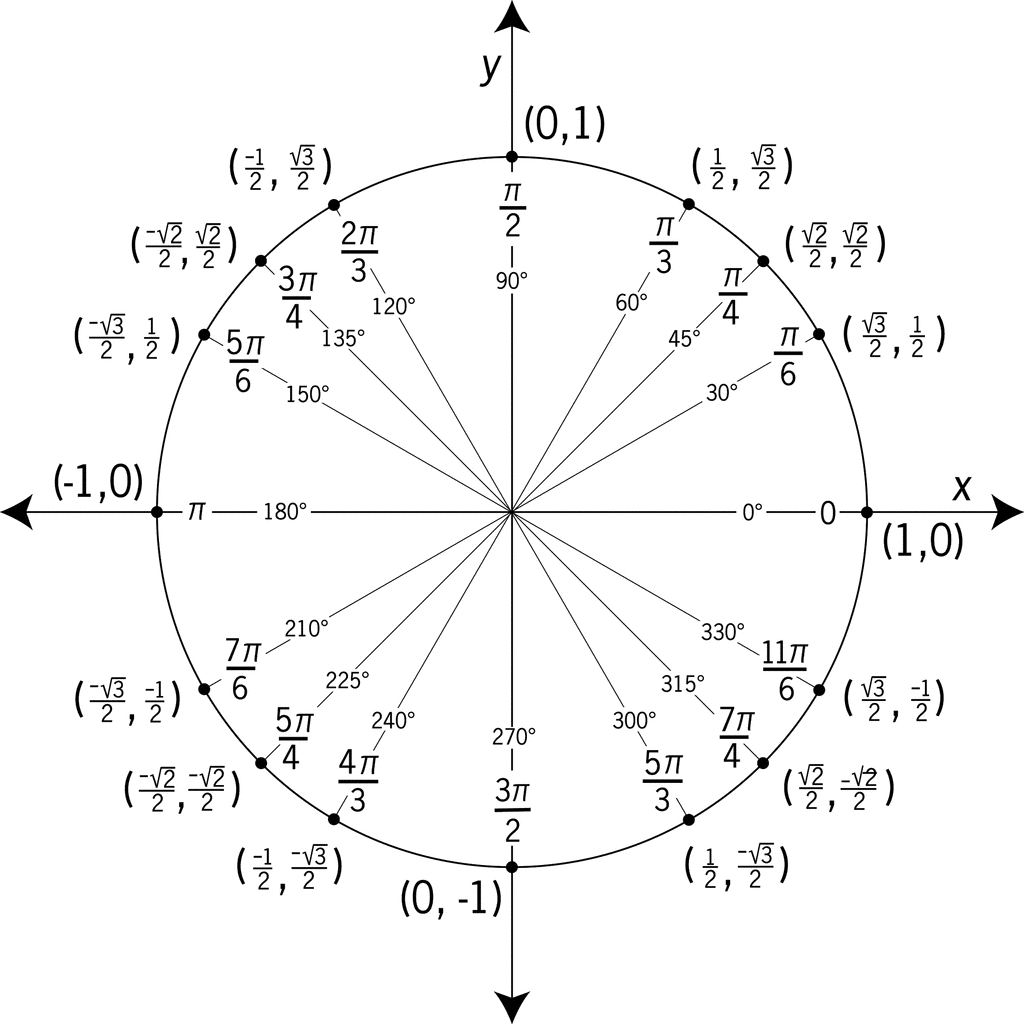
\includegraphics[width=0.8\textwidth]{unit-circle} %% SOURCE: http://etc.usf.edu
  \vfill
\end{center}


\pagebreak
\section{Goniometrische getallen van verwante hoeken}

\subsection{Gelijke hoeken}
We noemen twee hoeken $\alpha$ en $\beta$ \textbf{gelijk} als het maatgetal van $\alpha$ gelijk is aan het maatgetal van $\beta$.
\paragraph{}
Aangezien het maatgetal van een hoek slechts bepaald is op een geheel veelvoud van $360\degree$ zullen gelijke hoeken dezelfde goniometrische getallen hebben:
\begin{align*}
\sin(\alpha+k\cdot 360\degree)&=\sin(\alpha)\\
\cos(\alpha+k\cdot 360\degree)&=\cos(\alpha)\\
\tan(\alpha+k\cdot 360\degree)&=\tan(\alpha)\\
\cot(\alpha+k\cdot 360\degree)&=\cot(\alpha)\\
\end{align*}

\subsection{Tegengestelde hoeken}
\subsubsection*{Definitie}
We noemen twee hoeken $\alpha$ en $\beta$ \textbf{tegengesteld} als $\alpha=-\beta$.
\subsubsection*{Goniometrische getallen van tegengestelde hoeken}
Teken hieronder een goniometrische cirkel en lees erop af wat het verband is tussen $\sin(\alpha)$ en $\sin(-\alpha)$. Doe hetzelfde voor cos, tan en cot.
\vspace*{2cm}
\subsubsection*{Besluit}
\begin{align*}
  \sin(-\alpha)&=-\sin(\alpha)\\
  \cos(-\alpha)&=\cos(\alpha)\\
  \tan(-\alpha)&=-\tan(\alpha)\\
  \cot(-\alpha)&=-\cot(\alpha)
\end{align*}

\subsection{Complementaire hoeken}

\subsubsection*{Definitie}
We noemen twee hoeken $\alpha$ en $\beta$ \textbf{complementair} als hun som $90\degree$ is.

\subsubsection*{Goniometrische getallen van complementaire hoeken}
Teken hieronder een goniometrische cirkel en lees erop af wat het verband is tussen $\sin(\alpha)$ en $\sin(90\degree-\alpha)$. Doe hetzelfde voor cos, tan en cot.
\vspace*{7cm}

\subsubsection*{Besluit}
\begin{align*}
  \sin(90\degree-\alpha)&=\cos(\alpha)\\
  \cos(90\degree-\alpha)&=\sin(\alpha)\\
  \tan(90\degree-\alpha)&=\cot(\alpha)\\
  \cot(90\degree-\alpha)&=\tan(\alpha)
\end{align*}

\pagebreak
\subsection{Supplementaire hoeken}

\subsubsection*{Definitie}
We noemen twee hoeken $\alpha$ en $\beta$ \textbf{supplementair} als hun som $180\degree$ is.

\subsubsection*{Goniometrische getallen van supplementaire hoeken}
Teken hieronder een goniometrische cirkel en lees erop af wat het verband is tussen $\sin(\alpha)$ en $\sin(180\degree-\alpha)$. Doe hetzelfde voor cos, tan en cot.
\vspace*{7cm}
\subsubsection*{Besluit}
\begin{align*}
  \sin(180\degree-\alpha)&=\sin(\alpha)\\
  \cos(180\degree-\alpha)&=-\cos(\alpha)\\
  \tan(180\degree-\alpha)&=-\tan(\alpha)\\
  \cot(180\degree-\alpha)&=-\cot(\alpha)
\end{align*}

\pagebreak
\subsection{Anti-supplementaire hoeken}

\subsubsection*{Definitie}
We noemen twee hoeken $\alpha$ en $\beta$ \textbf{anti-supplementair} als verschil $180\degree$.

\subsubsection*{Goniometrische getallen van anti-supplementaire hoeken}
Teken hieronder een goniometrische cirkel en lees erop af wat het verband is tussen $\sin(\alpha)$ en $\sin(180\degree+\alpha)$. Doe hetzelfde voor cos, tan en cot.
\vspace*{6cm}

\subsubsection*{Besluit}
\begin{align*}
\sin(180\degree+\alpha)&=-\sin(\alpha)\\
\cos(180\degree+\alpha)&=-\cos(\alpha)\\
\tan(180\degree+\alpha)&=\tan(\alpha)\\
\cot(180\degree+\alpha)&=\cot(\alpha)  
\end{align*}

\pagebreak
\subsection{Oefeningen}

\begin{oefening}
Voor de hoek $\alpha$ van $135\degree$
\begin{enumerate}[(a)]
  \item Schets een goniometrische cirkel en duid hierop $\alpha$ aan.
  \item Duid $\sin \alpha$, $\cos \alpha$ en $\cot \alpha$ aan.
  \item Bereken $\sin \alpha$, $\cos \alpha$ en $\cot \alpha$ met behulp van verwante hoeken.
\end{enumerate}
\end{oefening}

\begin{oefening}
Bepaal de waarde van de volgende hoeken:
\begin{enumerate}[(a)]
  \itemsep.5em
  \item $\cos 150\degree$
  \item $\tan 300\degree$
  \item $\sin 315\degree$
  \item $\sec -60\degree$
  \item $\csc -30\degree$
\end{enumerate}
\end{oefening}

\begin{oefening}
Gegeven is dat de volgende vormen zinvol zijn. Schrijf ze zo eenvoudig mogelijk.
\begin{enumerate}[(a)]
  \itemsep1em
  \item $\dfrac{\cos(90\degree-\alpha)}{\tan(180\degree+\alpha)}$
  \item $\dfrac{\sin(90\degree-\alpha)}{\cot(180\degree-\alpha)}$
  \item $\dfrac{\sin(180\degree+\alpha).\tan(180\degree-\alpha)}{\tan(-\alpha)}$
  \item $(1-\cos(-\alpha)).(1+\cos(\alpha))$
  \item $\dfrac{\sin(90\degree-\alpha).\cos(360\degree+\alpha).\cot(90\degree-\alpha)}{\tan(180\degree-\alpha).\cot(\alpha+180\degree).\cos(-\alpha)}$
\end{enumerate}
\end{oefening}

\newpage
\section{Optellingsformules}

\subsection{Inleiding}
We willen een formule afleiden om de sinus, cosinus of tangens van een som van twee hoeken te berekenen:
\begin{align*}
  \sin(\alpha + \beta)\\
  \cos(\alpha + \beta)\\
  \tan(\alpha+\beta)
\end{align*}

Vul hiertoe de volgende uitdrukkingen aan en verbind wat aan elkaar gelijk is.

\begin{minipage}{0.4\textwidth}
  $$\sin(30\degree + 60\degree)=\arule{1cm}$$
\end{minipage}
\begin{minipage}{0.5\textwidth}
  $$\sin(30\degree) + \sin(60\degree)=\arule{1cm}$$
  $$\sin(30\degree)\cdot\cos(60\degree)+\cos(30\degree)\cdot\sin(60\degree)=\arule{1cm}$$
\end{minipage}

\begin{minipage}{0.4\textwidth}
  $$\sin(90\degree - 30\degree)=\arule{1cm}$$
\end{minipage}
\begin{minipage}{0.5\textwidth}
  $$\sin(90\degree) + \sin(30\degree)=\arule{1cm}$$
  $$\sin(90\degree)\cdot\cos(30\degree)-\cos(90\degree)\cdot\sin(30\degree)=\arule{1cm}$$
\end{minipage}

\begin{minipage}{0.4\textwidth}
  $$\cos(30\degree + 60\degree)=\arule{1cm}$$
\end{minipage}
\begin{minipage}{0.5\textwidth}
  $$\cos(30\degree) + \cos(60\degree)=\arule{1cm}$$
  $$\cos(30\degree)\cdot\cos(60\degree)-\sin(30\degree)\cdot\sin(60\degree)=\arule{1cm}$$
\end{minipage}

\begin{minipage}{0.4\textwidth}
  $$\cos(90\degree - 30\degree)=\arule{1cm}$$
\end{minipage}
\begin{minipage}{0.5\textwidth}
  $$\cos(90\degree) - \cos(30\degree)=\arule{1cm}$$
  $$\cos(90\degree)\cdot\cos(30\degree)-\sin(90\degree)\cdot\sin(30\degree)=\arule{1cm}$$
\end{minipage}



\subsection{Optellingsformules voor sinus en cosinus}

\subsubsection*{Besluit}
\begin{align*}
  \sin(\alpha + \beta)&=\sin(\alpha)\cdot \cos(\beta)+\cos(\alpha)\cdot \sin(\beta)\\
  \sin(\alpha - \beta)&=\sin(\alpha)\cdot \cos(\beta)-\cos(\alpha)\cdot \sin(\beta)\\
  \cos(\alpha + \beta)&=\cos(\alpha)\cdot \cos(\beta)-\sin(\alpha)\cdot \sin(\beta)\\
  \cos(\alpha - \beta)&=\cos(\alpha)\cdot \cos(\beta)+\sin(\alpha)\cdot \sin(\beta)
\end{align*}


\subsubsection*{Voorbeelden}

  \begin{enumerate}[(a)]
    \item Bereken $\sin(75\degree)$:
    \begin{align*}
      \sin(75\degree)&=\sin(45\degree+30\degree)\\
                     &=\sin(45\degree+30\degree)\\
                     &=\sin(45\degree)\cdot \cos(30\degree)+\cos(45\degree)\cdot \sin(30\degree)\\
                     &=\frac{\sqrt{2}}{2}\cdot \frac{\sqrt{3}}{2}+\frac{\sqrt{2}}{2}\cdot\frac{\sqrt{1}}{2}\\
                     &=\frac{\sqrt{6}+\sqrt{2}}{4}
    \end{align*}
    \item Vereenvoudig $\cos(4x)\cdot \cos(3x)-\sin(4x)\cdot \sin(3x)$
    \begin{align*}
      \cos(4x)\cdot \cos(3x)-\sin(4x)\cdot \sin(3x)&=\cos(3x+4x)\\
                                                   &=\cos(7x)
    \end{align*}
  \end{enumerate}

\begin{oefening}
Bereken $\cos(15\degree)$
\end{oefening}

\begin{oefening}
Vereenvoudig $\cos(19x)\cdot \cos(7x)+\sin(19x)\cdot \sin(7x)$
\end{oefening}

\pagebreak
\subsection{Optellingsformules voor tangens}
Uitgaande van deze formules leiden we nu een formule af voor de tangens van een som van 2 hoeken.

\subsubsection*{Opstellen formule}
\begin{align*}
  \tan(\alpha + \beta) &= \dfrac{\sin(\alpha + \beta)}{\cos(\alpha+\beta)}\\
                       &= \dfrac{\sin(\alpha)\cdot \cos(\beta)+\cos(\alpha)\cdot \sin(\beta)}{\cos(\alpha)\cdot \cos(\beta)-\sin(\alpha)\cdot \sin(\beta)}\\
                       &= \dfrac{\dfrac{\sin\alpha\cdot\cos\beta}{\cos\alpha\cdot\cos\beta}+\dfrac{\cos\alpha\cdot\sin\beta}{\cos\alpha\cdot\cos\beta}}{\dfrac{\cos\alpha\cdot\cos\beta}{\cos\alpha\cdot\cos\beta}+\dfrac{\sin\alpha\cdot\sin\beta}{\cos\alpha\cdot\cos\beta}}\\
                       &= \dfrac{\tan\alpha+\tan\beta}{1-\tan\alpha\cdot\tan\beta}
\end{align*}

In deze formule moeten $\alpha\neq 90\degree + k\cdot 180\degree$ en $\beta \neq 90\degree + k\cdot 180\degree$ teneinde te beletten dat $\tan\alpha$ en $\tan\beta$ niet zouden bestaan!

We spreken af om enkel hoeken te gebruiken waarvoor de gegeven vormen zinvol zijn. Er geldt ook:
\begin{align*}
  \tan(\alpha - \beta) &= \tan(\alpha + (-\beta))\\
                       &= \dfrac{\tan\alpha + \tan(-\beta)}{1-\tan\alpha\cdot\tan(-\beta)}\\
                       &= \dfrac{\tan\alpha - \tan\beta}{1+\tan\alpha\cdot\tan\beta}
\end{align*}

\subsubsection*{Besluit}
\begin{align*}
  \tan(\alpha + \beta)&=\frac{\tan(\alpha)+\tan(\beta)}{1-\tan(\alpha)\cdot\tan(\beta)}\\
  \tan(\alpha - \beta)&=\frac{\tan(\alpha)-\tan(\beta)}{1+\tan(\alpha)\cdot\tan(\beta)}
\end{align*}
\textbf{\[
\]}

\pagebreak
\subsubsection*{Voorbeelden}
Bereken
\begin{enumerate}[(a)]
  \item $\tan(60\degree - 30\degree)$
  \vspace*{-0.5cm}
  \begin{align*}
    \tan(60\degree - 30\degree)&=\dfrac{\tan(60\degree)-\tan(30\degree)}{1+\tan(60\degree)\cdot\tan(30\degree)}\\
                               &=\dfrac{\sqrt{3}-\frac{\sqrt{3}}{3}}{1+\sqrt{3}\cdot\frac{\sqrt{3}}{3}}\\
                               &=\dfrac{\frac{2}{3}\cdot\sqrt{3}}{2}\\
                               &=\dfrac{\sqrt{3}}{3}
  \end{align*}
  \item $\tan(75\degree)$
  \vspace*{-0.5cm}
  \begin{align*}
    \tan(75\degree) &= \tan(45\degree + 30\degree)\\
                    &= \dfrac{\tan45\degree+\tan30\degree}{1-\tan45\degree\cdot\tan30\degree}\\
                    &= \dfrac{1+\frac{\sqrt{3}}{3}}{1-1\cdot\frac{\sqrt{3}}{3}}\\
                    &= \ldots\\
                    &= 2+\sqrt{3}
  \end{align*}
\end{enumerate}


\subsection{Oefeningen}

\begin{oefening}
Bereken
\begin{enumerate}[(a)]
  \item $\cos(75\degree)$
  \item $\sin(15\degree)$
  \item $\tan(105\degree)$
\end{enumerate}
\end{oefening}

\begin{oefening}
Vereenvoudig
\begin{enumerate}[(a)]
  \item $\sin\frac{2x}{3}\cdot \cos\frac{x}{6}-\cos\frac{2x}{3}\cdot \sin\frac{x}{6}$
  \item $\cos\frac{8x}{5}\cdot \cos\frac{x}{10}+\sin\frac{8x}{5}\cdot \sin\frac{x}{10}$
  \item $\cos(110\degree)\cdot \cos(50\degree)+\sin(110\degree)\cdot \sin(50\degree)$
  \item $\sin(72\degree)\cdot \cos(27\degree)-\cos(72\degree)\cdot \sin(27\degree)$
\end{enumerate}
\end{oefening}

\begin{oefening}
Bewijs $\displaystyle \cot(\alpha+\beta)=\dfrac{\cot\alpha\cdot\cot\beta-1}{\cot\alpha+\cot\beta}$.
\end{oefening}

\newpage
\section{Formules van Simpson}
Uit de optellingsformules kunnen we formules afleiden die een product van sinussen en/of cosinussen omzetten in een som en omgekeerd.
\subsection{Eerste vorm van de formules van Simpson: product omzetten naar som}
\[2\cdot \sin(\alpha)\cdot \cos(\beta)=\sin(\alpha-\beta)+\sin(\alpha+\beta)
\]
\[2\cdot \cos(\alpha)\cdot \cos(\beta)=\cos(\alpha-\beta)+\cos(\alpha+\beta)
\]
\[2\cdot \sin(\alpha)\cdot \sin(\beta)=\cos(\alpha-\beta)-\cos(\alpha+\beta)
\]

\subsubsection*{Voorbeelden}

\begin{enumerate}[(1)]
  \item\underline{Schrijf als som}
    \begin{enumerate}[(a)]
      \item $2\cdot \sin(3x)\cdot \cos(2x)= $\dotfill
      \item $2\cdot \cos(4x)\cdot \cos(2x)= $\dotfill
      \item $2\cdot \sin(5x)\cdot \sin(x)= $\dotfill
      \item $2\cdot \sin(x)\cdot \cos(3x)= $\dotfill
      \item $\cos(3x)\cdot \cos(2x)= $\dotfill
      \item $\sin(3x)\cdot \sin(-3x)= $\dotfill
    \end{enumerate}
  \item \underline{Bereken exact}
    \begin{enumerate}[(a)]
      \item $2\cdot \cos(75\degree)\cdot \cos(15\degree) = \dotfill \newline =$\dotfill
      \item $2\cdot \sin(75\degree)\cdot \cos(15\degree) = \dotfill \newline =$\dotfill
      \item $2\cdot \sin(\frac{5\pi}{12})\cdot \sin(\frac{\pi}{12}) = $\dotfill \newline =\dotfill
      \item $2\cdot \cos(120\degree)\cdot \cos(60\degree) = $\dotfill \newline =\dotfill
    \end{enumerate}
\end{enumerate}

\newpage
\subsection{Tweede vorm van de formules van Simpson: som onzetten naar product}
\[\sin(p)+\sin(q)=2\cdot \sin(\frac{p+q}{2})\cdot \cos(\frac{p-q}{2})
\]
\[\sin(p)-\sin(q)=2\cdot \cos(\frac{p+q}{2})\cdot \sin(\frac{p-q}{2})
\]
\[\cos(p)+\cos(q)=2\cdot \cos(\frac{p+q}{2})\cdot \cos(\frac{p-q}{2})
\]
\[\cos(p)-\cos(q)=-2\cdot \sin(\frac{p+q}{2})\cdot \sin(\frac{p-q}{2})
\]

\subsubsection*{Voorbeelden}

\begin{enumerate}[(1)]
  \item\underline{Schrijf als product}
    \begin{enumerate}[(a)]
      \item $\cos5x+\cos x=$ \dotfill
      \item $\cos x-\cos17x=$ \dotfill
      \item $\sin8x+\sin2x=$ \dotfill
      \item $\cos(\frac{\pi}{5})+\cos(\frac{\pi}{7})=$ \dotfill
    \end{enumerate}
  \item \underline{Bereken exact}
    \begin{enumerate}[(a)]
      \item $\sin(75\degree)+\sin(15\degree) =$ \dotfill \newline =\dotfill
      \item $\cos(75\degree)+\cos(15\degree) =$ \dotfill \newline =\dotfill
      \item $\cos(\frac{-\pi}{12})-\cos(\frac{7\pi}{12}) =$ \dotfill \newline =\dotfill
    \end{enumerate}
\end{enumerate}

%\newpage
\end{document}
